In deze kwaliteitscontrole worden enkele testen beschreven. Deze rubriek somt als het ware de verschillende testplannen op. Er wordt telkens wat uitleg gegeven over de gebruikte aanpakt gevolgd door een beschrijving of een uitvoering van dergelijke test. 

\subsection{Overzicht Testplan}

De unit testen zullen vooral de business logica van de verschillende use cases testen op een mock data laag met testgegevens. Hierdoor zijn de testgegevens steeds hetzelfde en kan bij aanpassingen aan de services gemakkelijk geverifiëerd worden of er geen bugs geintroduceerd zijn.

De integration tests testen de verbinding met de database en de stabiele werking van het systeem in het algemeen. Ook hier wordt gebruik gemaakt van de main flows van de belangrijkse use cases.

Tenslotte testen de usability testen de algemene gebruiksvriendelijkheid van de applicatie, o.a of het voor een leek die niet vertrouwd is met het systeem vlug duidelijk is waar alles te vinden is en hoe gemakkelijk hij/zij het vindt om bepaalde gegevens op te vragen. Verder wordt er ook gekeken naar de performantie en responsiviteit van de applicatie door heel veel data in de databank te steken en te kijken of er geen vertragingen naar boven komen.

\subsection{Unit Tests}

Om zeker te zijn dat bepaalde algoritmes van het project correct werken, worden er unit testen aangemaakt. Om maximaal rendement uit de unit testen te halen, worden er geen triviale testen gemaakt voor bijvoorbeeld setters zonder logica. Er zal gebruik gemaakt worden van het framework Mockito om dependecies te mocken en JUnit voor de testen. 

De belangrijkste algoritmes die getest moeten worden zijn:

\begin{itemize}
\item Het detecteren van extreme providers op de detail page (door Aaron).
\item Het gemiddelde berekenen van een route over een bepaalde periode en enkel voor bepaalde providers (door Aaron).
\item Het detecteren van files (door Dwight).
\end{itemize}

\subsection{Integration Tests (via Selenium)}

Het is een discussiepunt om de functionele acceptatie-testen van selenium nu al dan niet te categoriseren onder integratietesten. Omdat de testen toch wel data van backend ophalen via de frontend alsof ze een gebruiker zijn hebben we toch gekozen om deze hier te plaatsen. Een correctere term is waarschijnlijk smoke of sanity test.

Selenium IDE is een plugin waarmee je browseractiviteiten kan opnemen. Men kan elementen op de webapplicatie selecteren en deze controleren. Na het opnemen kan zo'n test case (of suite) geëxporteerd worden naar testen die uitgevoerd kunnen worden in bijvoorbeeld JUnit.

Een voorbeeld van zo'n test is het ophalen en controleren (via regex momenteel) of elke route wel een acceptabele normale reistijd, huidige reistijd en vertraging heeft. 

Een demo en voorbeeld zijn te zien op \url{https://www.youtube.com/watch?v=8HOH1TDGWdo}.

\subsection{Usability Tests (Use case testing)}

Met use case testing bedoelt men soms het ``het maken van'' use cases in een Agile of TDD (Test Driven Development)-omgeving. In deze rubriek hebben we echter de use cases genomen en deze omgezet in een stappenplan. Het doornemen van deze stappen test zo onze applicatie aan onze use cases. Op die manier worden de gewenste doelstelling getest en worden ook de use cases deel van de documentatie van het eindproduct.

Bij het maken van het stappenplan hebben we geprobeerd alles te schrijven vanuit de gebruike zijn standpunt. Om die reden zijn er enkele use cases die niet (rechtstreeks) getest kunnen worden door de gebruiker. Men zou alternatieven kunnen voorzien maar dit is niet echt nodig. In deze use cases worden alle gegevens verzamelt en weggeschreven naar de databank. Deze use cases zijn dan ook niet echt bedoelt om te testen in een usability test. SQL-queries of inloggen op de server en onze testscrips runnen zijn workarounds. Het is echter zo dat als de andere use case die getest worden aan de hand van usability tests (ook) gaan falen als deze use cases niet correct zijn. Daarom mogen we concluderen dat deze use cases correct doorloopbaar zijn zonder expliciet een stappenplan te volgen. 

\begin{itemize}
\item Uc: Verzamelen POI-gegevens
\item Uc: Verzamelen weergevens
\item Uc: Verzamel reistijdgegevens
\end{itemize}

Volgende 2 tabellen toont het stappenplan die opgemaakt werd op basis van de use cases. We doorlopen het stap voor stap een\, \cmark \, toont aan dat alles geslaagd is terwijl een\, \xmark \, aantoont dat er nog iets niet in orde is.

\begin{table}[H]
\centering
\begin{tabular}{|r|l|l|}
\hline
\multicolumn{3}{|c|}{{\textbf{UC: Bekijk routeoverzicht}}}                         \\ \hline
\multicolumn{1}{|c|}{Stappenplan:} &                                            &  \\ \hline
1.                                 & Gebruiker gaat naar de website.            & \cmark \\ \hline
2.                                 & Gebruiker kan op routeoverzicht klikken.   & \cmark \\ \hline
3.                                 & Een overzicht van de routes wordt getoond. & \cmark \\ \hline
4.                                 & Een overzicht van de routes wordt getoond. & \cmark \\ \hline
\multicolumn{3}{|c|}{{\textbf{UC: Bekijk routedetail}}}                            \\ \hline
\multicolumn{1}{|c|}{Stappenplan:} &                                            &  \\ \hline
1.                                 & Gebruiker gaat naar de website.            & \cmark \\ \hline
2.                                 & Gebruiker kan op routeoverzicht klikken.   & \cmark \\ \hline
3.                                 & Gebruiker kan op een route klikken voor de details. & \cmark \\ \hline
4.                                 & De routedetails worden getoond.            & \cmark \\ \hline
\multicolumn{3}{|c|}{{\textbf{UC: Bekijk routemap}}}                          \\ \hline
\multicolumn{1}{|c|}{Stappenplan:} &                                            &  \\ \hline
1.                                 & Gebruiker gaat naar de website.            & \cmark \\ \hline
2.                                 & Gebruiker kan op routemap klikken.   & \cmark \\ \hline
3.                                 & De routemap wordt getoond.        & \cmark \\ \hline
\multicolumn{3}{|c|}{{\textbf{UC: Vergelijk providerdata}}}                            \\ \hline
\multicolumn{1}{|c|}{Stappenplan:} &                                            &  \\ \hline
1.                                 & Gebruiker gaat naar de website.            & \cmark \\ \hline
2.                                 & Gebruiker kan op routeoverzicht klikken.   & \cmark \\ \hline
3.                                 & Gebruiker kan op een route klikken voor de details. & \cmark \\ \hline
4.                                 & Gebruiker kan providerdata vergelijken.            & \cmark \\ \hline
\multicolumn{3}{|c|}{{\textbf{UC: Wijzig route}}}                            \\ \hline
\multicolumn{1}{|c|}{Stappenplan:} &                                            &  \\ \hline
1.                                 & Gebruiker gaat naar de website.            & \cmark \\ \hline
2.                                 & Gebruiker kan op routeoverzicht klikken.   & \cmark \\ \hline
3.                                 & Gebruiker kan op wijzig klikken. & \cmark \\ \hline
4.                                 & Gebruiker kan de details van de route wijzigen.            & \cmark \\ \hline
\multicolumn{3}{|c|}{{\textbf{UC: Logpagina bekijken}}}                            \\ \hline
\multicolumn{1}{|c|}{Stappenplan:} &                                            &  \\ \hline
1.                                 & Gebruiker gaat naar de website.            & \cmark \\ \hline
2.                                 & Gebruiker kan op logpagina klikken.   & \xmark \\ \hline
\end{tabular}
\caption{Usability Tests (use case testing (1/2)}
\end{table}

\begin{table}[H]
\centering
\begin{tabular}{|r|l|l|}
\hline
\multicolumn{3}{|c|}{{\textbf{UC: Dashboard bekijken}}}                         \\ \hline
\multicolumn{1}{|c|}{Stappenplan:} &                                            &  \\ \hline
1.                                 & Gebruiker gaat naar de website.            & \cmark \\ \hline
2.                                 & Gebruiker kan dashboard(s) bekijken.       & \cmark \\ \hline
\multicolumn{3}{|c|}{{\textbf{UC: Aanbieden routegegevens met reistijden.}}}                            \\ \hline
\multicolumn{1}{|c|}{Stappenplan:} &                                            &  \\ \hline
1.                                 & Gebruiker maakt een specifieke request.            & \xmark \\ \hline
2.                                 & De gebruiker krijgt correcte gegevens naar gelang de request.   & \xmark \\ \hline
\multicolumn{3}{|c|}{{\textbf{UC: Vergelijk routes}}}                          \\ \hline
\multicolumn{1}{|c|}{Stappenplan:} &                                            &  \\ \hline
1.                                 & Gebruiker gaat naar de website.            & \xmark \\ \hline
2.                                 & Gebruiker klikt op vergelijk routes.   & \xmark \\ \hline
3.                                 & Gebruiker geeft routedetails op.       & \xmark \\ \hline
4.                                 & Een grafiek wordt getoond waarin de routes vergeleken kunnen worden.       & \xmark \\ \hline
\end{tabular}
\caption{Usability Tests (use case testing (2/2)}
\end{table}

Bovenstaande stappen werden overlopen op 16 april. Alle zaken die falen zijn nog geplande, niet-geïmplementeerde features. 


\subsection{Usability Tests (scenario)}


Deze manueel uitgevoerde scenarios dienen de usability and user experience (UX) te testen. Er werd aan 3 personen gevraagd om een specifiek scenario door te nemen. De testpersonen moeten aanduiden of ze de verschillende stappen van het scenario goed kunnen uitvoeren of niet, alsook het loggen van de gespendeerde tijd. Het uitvoeren van de verschillende stappen test als gevolg het gebruik van de applicatie. Tot slot werd er gevraagd aan de testpersonen of ze nog opmerkingen, vragen of onduidelijkheden hadden.

Er werd geopteerd om 3 profielen te benaderen. Onze keuze is uitgegaan naar een IT-deskundige en 2 niet-IT-deskundigen. Deze laatste groep verschilt dan nog eens in leeftijd (enederzijds $\pm 20$ jaar en anderzijds  $\pm 50$ jaar).

Er is 1 use case die we zelf uitvoerig gebruikt (en dus getest hebben) en dat is ``route wijzigen''. Het sprekt ook voor zich dat we op de productieomgeving deze use case liever niet laten derden doornemen door derden. ``De vergelijk routes''-use case is bovendien nog niet geïmplementeerd.

% Dit is getest en in orde:
% Ik kan een route wijzigen.

% Not implemented yet:

% Setting pagina
% Compare pagina
% Bij het invoeren van een verkeerde url op domein krijg ik een correcte errorpagina.

\newpage

\subsubsection{Template}

Het scenario (of stappenplan) dat werd gegeven aan de testpersonen ziet er als volgt uit:

\begin{table}[H]
\centering
\begin{tabular}{|r|l|l|l|l|l|}
\hline
\multicolumn{1}{|c|}{\textit{\textbf{Stap}}} & \multicolumn{1}{c|}{\textit{\textbf{Beschrijving}}}                                                                    & \multicolumn{1}{c|}{\textit{\textbf{Ok}}} & \multicolumn{1}
{c|}{\textit{\textbf{Ind.}}} & \multicolumn{1}
{c|}{\textit{\textbf{Cum.}}} \\ \hline
1 & \multicolumn{1}{p{9cm}|}{Ik kan naar de website: \url{http://verkeer-4.vop.tiwi.be/} surfen en inloggen met de credentials guest/1RRBpmM0KC.} & \multicolumn{1}{c|}{}                         &  &  \\ \hline

2 & \multicolumn{1}{p{9cm}|}{Ik kan het weer aflezen van de website.} & \multicolumn{1}{c|}{}     
&  &  \\ \hline

3 & \multicolumn{1}{p{9cm}|}{Ik kan de laatste tweets van ``VerkeerGentB'' zien.} & \multicolumn{1}{c|}{}   
&  &  \\ \hline

4 & \multicolumn{1}{p{9cm}|}{Ik kan een overzicht van alle routes zien met hun afstanden, standaardtijden, huidige reistijden en huidige vertragingen.} & \multicolumn{1}{c|}{}      
&  &  \\ \hline

5 & \multicolumn{1}{p{9cm}|}{Ik kan naar een route gaan en zijn weg visueel zien op een kaart.} & \multicolumn{1}{c|}{}      
&  &  \\ \hline

6 & \multicolumn{1}{p{9cm}|}{Ik kan de vertraging van Bing op Paryslaan (R4) northbound te weten komen.} & \multicolumn{1}{c|}{}      
&  &  \\ \hline

7 & \multicolumn{1}{p{9cm}|}{Ik kan een visueel overzicht krijgen op de kaart waar er momenteel vertragingen zijn.} & \multicolumn{1}{c|}{}      
&  &  \\ \hline

8 & \multicolumn{1}{p{9cm}|}{Ik kan visueel zien of er zich ergens probleempunten vertonen in de buurt van Gent.} & \multicolumn{1}{c|}{}      
&  &  \\ \hline

9 & \multicolumn{1}{p{9cm}|}{Ik kan te weten komen wat de huidige reistijd was per provider op 17 maart tussen 6:00 en 11:00 in de Rooigemlaan (R40) northbound.} & \multicolumn{1}{c|}{}      
&  &  \\ \hline

10 & \multicolumn{1}{p{9cm}|}{Ik kan te weten komen wat de vertraging was per provider op 17 maart tussen 6:00 en 11:00 in de Rooigemlaan (R40) northbound.} & \multicolumn{1}{c|}{}      
&  &  \\ \hline

11 & \multicolumn{1}{p{9cm}|}{Ik kan de data van vorige test opslaan als in een csv-bestand (te openen met excel).} & \multicolumn{1}{c|}{}      
&  &  \\ \hline

12 & \multicolumn{1}{p{9cm}|}{Ik kan te weten komen welke route volgens google het meeste vertraging heeft.} & \multicolumn{1}{c|}{}      
&  &  \\ \hline

13 & \multicolumn{1}{p{9cm}|}{Ik kan te weten komen welke route de grootste afstand heeft.} & \multicolumn{1}{c|}{}      
&  &  \\ \hline

\end{tabular}
\caption{Scenario Usability Test Template}
\end{table}


\subsubsection{Persoon 1: IT-deskundige}

\begin{table}[H]
\centering
\begin{tabular}{|r|l|l|l|l|}
\hline
\multicolumn{1}{|c|}{\textit{\textbf{Stap}}} & \multicolumn{1}{c|}{\textit{\textbf{Beschrijving}}}                                                                    & \multicolumn{1}{c|}{\textit{\textbf{Ok}}} & \multicolumn{1}
{c|}{\textit{\textbf{Ind.}}} & \multicolumn{1}
{c|}{\textit{\textbf{Cum.}}} \\ \hline
1 & \multicolumn{1}{p{9cm}|}{Ik kan naar de website: \url{http://verkeer-4.vop.tiwi.be/} surfen en inloggen met de credentials guest/1RRBpmM0KC.} & \multicolumn{1}{c|}{\cmark}                         & 00:30 & 00:30 \\ \hline

2 & \multicolumn{1}{p{9cm}|}{Ik kan het weer aflezen van de website.} & \multicolumn{1}{c|}{\cmark}     
& 00:05 & 00:35 \\ \hline

3 & \multicolumn{1}{p{9cm}|}{Ik kan de laatste tweets van ``VerkeerGentB'' zien.} & \multicolumn{1}{c|}{\cmark}   
& 00:00 & 00:35  \\ \hline

4 & \multicolumn{1}{p{9cm}|}{Ik kan een overzicht van alle routes zien met hun afstanden, standaardtijden, huidige reistijden en huidige vertragingen.} & \multicolumn{1}{c|}{\cmark}      
& 01:00 & 01:35  \\ \hline

5 & \multicolumn{1}{p{9cm}|}{Ik kan naar een route gaan en zijn weg visueel zien op een kaart.} & \multicolumn{1}{c|}{\cmark}      
& 01:00 & 02:35  \\ \hline

6 & \multicolumn{1}{p{9cm}|}{Ik kan de vertraging van Bing op Paryslaan (R4) northbound te weten komen.} & \multicolumn{1}{c|}{\cmark}      
& 02:00 & 04:35  \\ \hline

7 & \multicolumn{1}{p{9cm}|}{Ik kan een visueel overzicht krijgen op de kaart waar er momenteel vertragingen zijn.} & \multicolumn{1}{c|}{\cmark}      
& 01:00 & 05:35  \\ \hline

8 & \multicolumn{1}{p{9cm}|}{Ik kan visueel zien of er zich ergens probleempunten vertonen in de buurt van Gent.} & \multicolumn{1}{c|}{\cmark}      
& 00:00 & 05:35  \\ \hline

9 & \multicolumn{1}{p{9cm}|}{Ik kan te weten komen wat de huidige reistijd was per provider op 17 maart tussen 6:00 en 11:00 in de Rooigemlaan (R40) northbound.} & \multicolumn{1}{c|}{\cmark}      
& 02:00 & 07:35  \\ \hline

10 & \multicolumn{1}{p{9cm}|}{Ik kan te weten komen wat de vertraging was per provider op 17 maart tussen 6:00 en 11:00 in de Rooigemlaan (R40) northbound.} & \multicolumn{1}{c|}{\cmark}      
& 01:00 & 08:35  \\ \hline

11 & \multicolumn{1}{p{9cm}|}{Ik kan de data van vorige test opslaan als in een csv-bestand (te openen met excel).} & \multicolumn{1}{c|}{\cmark}      
& 00:05 & 08:40  \\ \hline

12 & \multicolumn{1}{p{9cm}|}{Ik kan te weten komen welke route volgens google het meeste vertraging heeft.} & \multicolumn{1}{c|}{\cmark}      
& 02:00 & 10:40  \\ \hline

13 & \multicolumn{1}{p{9cm}|}{Ik kan te weten komen welke route de grootste afstand heeft.} & \multicolumn{1}{c|}{\cmark}      
& 00:10 & 10:50  \\ \hline

\end{tabular}
\caption{Scenario Usability Test Persoon 1: IT-deskundige}
\end{table}

Opmerkingen:

\begin{itemize}
\item Onduidelijk navigatiemenu.
\item In het algemeen niet zo duidelijk als je niet doorklikt.
\item Zaken die nog niet geïmplementeerd zijn moeten er best nog niet op.
\end{itemize}

\subsubsection{Persoon 2: niet-IT-deskundige (1)}

\begin{table}[H]
\centering
\begin{tabular}{|r|l|l|l|l|}
\hline
\multicolumn{1}{|c|}{\textit{\textbf{Stap}}} & \multicolumn{1}{c|}{\textit{\textbf{Beschrijving}}}                                                                    & \multicolumn{1}{c|}{\textit{\textbf{Ok}}} & \multicolumn{1}
{c|}{\textit{\textbf{Ind.}}} & \multicolumn{1}
{c|}{\textit{\textbf{Cum.}}} \\ \hline
1 & \multicolumn{1}{p{9cm}|}{Ik kan naar de website: \url{http://verkeer-4.vop.tiwi.be/} surfen en inloggen met de credentials guest/1RRBpmM0KC.} & \multicolumn{1}{c|}{\cmark}                         & 00:40 & 00:40 \\ \hline

2 & \multicolumn{1}{p{9cm}|}{Ik kan het weer aflezen van de website.} & \multicolumn{1}{c|}{\cmark}     
& 00:05 & 00:45 \\ \hline

3 & \multicolumn{1}{p{9cm}|}{Ik kan de laatste tweets van ``VerkeerGentB'' zien.} & \multicolumn{1}{c|}{\cmark}   
& 00:00 & 00:45 \\ \hline

4 & \multicolumn{1}{p{9cm}|}{Ik kan een overzicht van alle routes zien met hun afstanden, standaardtijden, huidige reistijden en huidige vertragingen.} & \multicolumn{1}{c|}{\cmark}      
& 01:00 & 01:45 \\ \hline

5 & \multicolumn{1}{p{9cm}|}{Ik kan naar een route gaan en zijn weg visueel zien op een kaart.} & \multicolumn{1}{c|}{\cmark}      
& 00:30 & 02:15 \\ \hline

6 & \multicolumn{1}{p{9cm}|}{Ik kan de vertraging van Bing op Paryslaan (R4) northbound te weten komen.} & \multicolumn{1}{c|}{\cmark}      
& 01:00 & 03:15 \\ \hline

7 & \multicolumn{1}{p{9cm}|}{Ik kan een visueel overzicht krijgen op de kaart waar er momenteel vertragingen zijn.} & \multicolumn{1}{c|}{\cmark}      
& 01:00 & 04:15 \\ \hline

8 & \multicolumn{1}{p{9cm}|}{Ik kan visueel zien of er zich ergens probleempunten vertonen in de buurt van Gent.} & \multicolumn{1}{c|}{\cmark}      
& 00:00 & 04:15 \\ \hline

9 & \multicolumn{1}{p{9cm}|}{Ik kan te weten komen wat de huidige reistijd was per provider op 17 maart tussen 6:00 en 11:00 in de Rooigemlaan (R40) northbound.} & \multicolumn{1}{c|}{\cmark}      
& 01:30 & 05:45 \\ \hline

10 & \multicolumn{1}{p{9cm}|}{Ik kan te weten komen wat de vertraging was per provider op 17 maart tussen 6:00 en 11:00 in de Rooigemlaan (R40) northbound.} & \multicolumn{1}{c|}{\xmark}      
& 02:00 & 07:45 \\ \hline

11 & \multicolumn{1}{p{9cm}|}{Ik kan de data van vorige test opslaan als in een csv-bestand (te openen met excel).} & \multicolumn{1}{c|}{\cmark}      
& 00:30 & 08:15 \\ \hline

12 & \multicolumn{1}{p{9cm}|}{Ik kan te weten komen welke route volgens google het meeste vertraging heeft.} & \multicolumn{1}{c|}{\xmark}      
& 02:00 & 10:15 \\ \hline

13 & \multicolumn{1}{p{9cm}|}{Ik kan te weten komen welke route de grootste afstand heeft.} & \multicolumn{1}{c|}{\cmark}      
& 00:30 & 10:45 \\ \hline

\end{tabular}
\caption{Scenario Usability Test Persoon 2: niet-IT-deskundige (1)}
\end{table}

Opmerkingen:

\begin{itemize}
\item Bij het weer wordt niet aangegeven dat dit van Gent is.
\item CTT en D is niet duidelijk voor personen die er niet mee bezig zijn.
\item Er zou een duidelijkere scheiding moeten zijn tussen de providers vanboven omdat het niet duidelijk is welke CTT en D bij welke provider horen.
\item Sorteren niet duidelijk.
\end{itemize}

\subsubsection{Persoon 3: niet-IT-deskundige (2)}

\begin{table}[H]
\centering
\begin{tabular}{|r|l|l|l|l|}
\hline
\multicolumn{1}{|c|}{\textit{\textbf{Stap}}} & \multicolumn{1}{c|}{\textit{\textbf{Beschrijving}}}                                                                    & \multicolumn{1}{c|}{\textit{\textbf{Ok}}} & \multicolumn{1}
{c|}{\textit{\textbf{Ind.}}} & \multicolumn{1}
{c|}{\textit{\textbf{Cum.}}} \\ \hline
1 & \multicolumn{1}{p{9cm}|}{Ik kan naar de website: \url{http://verkeer-4.vop.tiwi.be/} surfen en inloggen met de credentials guest/1RRBpmM0KC.} & \multicolumn{1}{c|}{\cmark}                         & 01:40 & 01:40 \\ \hline

2 & \multicolumn{1}{p{9cm}|}{Ik kan het weer aflezen van de website.} & \multicolumn{1}{c|}{\cmark}     
& 00:10 & 01:50 \\ \hline

3 & \multicolumn{1}{p{9cm}|}{Ik kan de laatste tweets van ``VerkeerGentB'' zien.} & \multicolumn{1}{c|}{\cmark}   
& 00:10 & 02:00 \\ \hline

4 & \multicolumn{1}{p{9cm}|}{Ik kan een overzicht van alle routes zien met hun afstanden, standaardtijden, huidige reistijden en huidige vertragingen.} & \multicolumn{1}{c|}{\cmark}      
& 01:00 & 03:00 \\ \hline

5 & \multicolumn{1}{p{9cm}|}{Ik kan naar een route gaan en zijn weg visueel zien op een kaart.} & \multicolumn{1}{c|}{\cmark}      
& 00:30 & 03:30 \\ \hline

6 & \multicolumn{1}{p{9cm}|}{Ik kan de vertraging van Bing op Paryslaan (R4) northbound te weten komen.} & \multicolumn{1}{c|}{\cmark}      
& 02:00 & 05:30 \\ \hline

7 & \multicolumn{1}{p{9cm}|}{Ik kan een visueel overzicht krijgen op de kaart waar er momenteel vertragingen zijn.} & \multicolumn{1}{c|}{\cmark}      
& 01:00 & 06:30 \\ \hline

8 & \multicolumn{1}{p{9cm}|}{Ik kan visueel zien of er zich ergens probleempunten vertonen in de buurt van Gent.} & \multicolumn{1}{c|}{\cmark}      
& 00:10 & 06:40 \\ \hline

9 & \multicolumn{1}{p{9cm}|}{Ik kan te weten komen wat de huidige reistijd was per provider op 17 maart tussen 6:00 en 11:00 in de Rooigemlaan (R40) northbound.} & \multicolumn{1}{c|}{\cmark}      
& 02:30 & 09:10 \\ \hline

10 & \multicolumn{1}{p{9cm}|}{Ik kan te weten komen wat de vertraging was per provider op 17 maart tussen 6:00 en 11:00 in de Rooigemlaan (R40) northbound.} & \multicolumn{1}{c|}{\xmark}      
& 02:30 & 11:40 \\ \hline

11 & \multicolumn{1}{p{9cm}|}{Ik kan de data van vorige test opslaan als in een csv-bestand (te openen met excel).} & \multicolumn{1}{c|}{\cmark}      
& 01:00 & 12:40 \\ \hline

12 & \multicolumn{1}{p{9cm}|}{Ik kan te weten komen welke route volgens google het meeste vertraging heeft.} & \multicolumn{1}{c|}{\xmark}      
& 02:30 & 15:10 \\ \hline

13 & \multicolumn{1}{p{9cm}|}{Ik kan te weten komen welke route de grootste afstand heeft.} & \multicolumn{1}{c|}{\cmark}      
& 01:00 & 16:10 \\ \hline

\end{tabular}
\caption{Scenario Usability Test Persoon 3: niet-IT-deskundige (2)}
\end{table}

Opmerkingen:

\begin{itemize}
\item CTT en D is niet duidelijk voor personen die er niet mee bezig zijn.
\item Er zou een duidelijkere scheiding moeten zijn tussen de providers vanboven omdat het niet duidelijk is welke CTT en D bij welke provider horen.
\item Sorteren niet duidelijk.
\item Opslaan is niet duidelijk aangegeven.
\end{itemize}



\newpage

\subsection{Load Tests (via Apache JMeter)}

% Algemene uitleg:

% Number of threats -> en loops (wij altijd 1 keer)

% Ramp-up needs to be long enough to avoid too large a work-load at the start of a test, and short enough that the last threads start running before the first ones finish (unless one wants that to happen).

Apache JMeter is een load testing tool waarin je users kan simuleren voor je webapplicatie. In de vorm van threads worden zo HTTP Requests uitgevoerd naar de verschillende pagina's. Op die manier kan men vrij snel een server testen tegen veel verkeer.

We hebben drie testen voorzien. De eerste bezoekt enkel de homepagina (en vult de basic auth correct in). De tweede gaat vervolgens nog naar de map view en de derde simuleert een volwaardige gebruiker die van het dashboard naar de overview surft om nadien een route te selecteren die hij in detail wil bekijken. De testen worden lokaal uitgevoerd tegen de productieserver. 

Een demo is te vinden in de vorm van een filmpje: \url{https://www.youtube.com/watch?v=h2HiMyBYgCI}.


\begin{figure}[H]
\centering
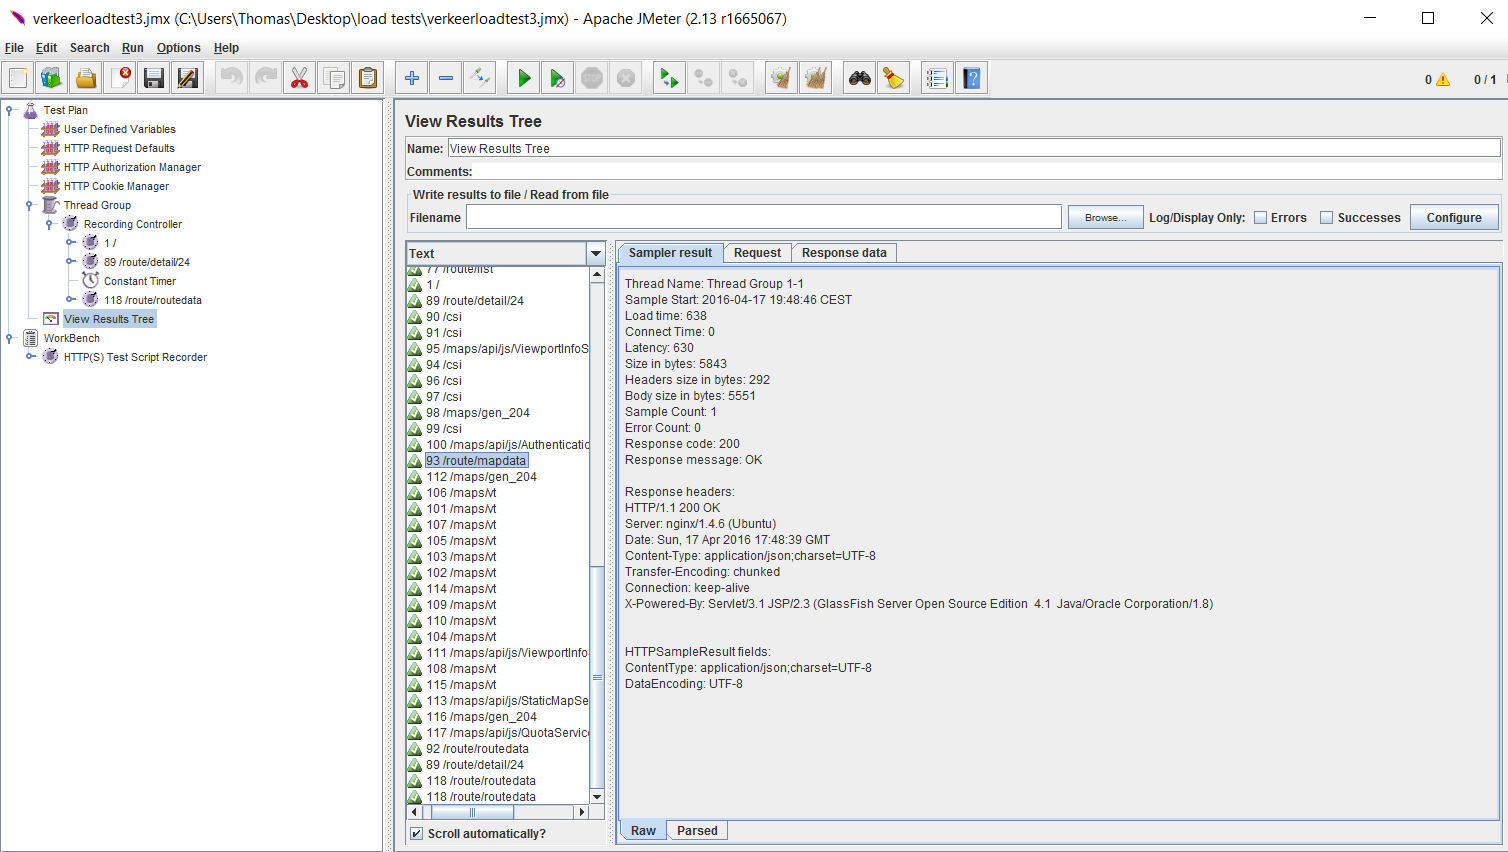
\includegraphics[width=\textwidth]{images/jmeterexample.png}\\
\caption{Apache JMeter - Voorbeeld}
\end{figure}








